\section{Auswertung} 

\begin{flushleft}
    Gemessen wurden die Zeiten $\text{t}_{\text{ab}}$, $\text{t}_{\text{auf}}$ und $\text{t}_{0}$. 
    Dafür wurden die Platten umgepolt wie in Abbildung \ref{Abbildung1}. 
    Für die Gleichgewichtslage wurde keine Spannung angebracht.
    Die Tröpfchen wurden über eine Strecke von   $\text{s}= 0,5 \cdot 10^{-3}\,\unit{\meter}$ beobachtet.
    Die Zeiten wurden tabellarisch in Tabelle \ref{Tabelle1}, Tabelle \ref{Tabelle6}, und Tabelle \ref{Tabelle7} festgehalten. 
\end{flushleft}

\begin{table} [H]
    \caption{Gemessene Zeiten (1)}
    \label{Tabelle1}
    \begin{subtable}[c]{0.5\textwidth}
    \centering
    \caption{$\text{U} = 190\,\text{V}, \text{R} = 2,27\,\unit{\mega\ohm}, \text{T} = 20\unit{\celsius}  $}
    \begin{tabular}{ c|c|c}
        \toprule
        {$\text{t}_{0} \mathbin{/}\unit{\second} $}&
        {$\text{t}_{\text{auf}} \mathbin{/}\unit{\second} $}&
        {$\text{t}_{\text{ab}} \mathbin{/}\unit{\second} $}\\
        \midrule
        63  & 2,04 & 1,94 \\
            & 1,86 & 2,27 \\
            & 1,68 & 1,84 \\
            & 2,04 & 1,72 \\
        \rowcolor{gray}$\to$ & $1,90 \pm 0,17$ & $1,94 \pm 0,23$ \\
            &  &  \\
        42,32 & 5,25 & 3,82\\
            & 4,32 & 4,18 \\
            & 4,76 & 4,24\\
            & 4,70 & 3,97 \\
        \rowcolor{gray}$\to$ & $4,74 \pm 0,33$ & $4,05 \pm 0,16$ \\
            &  &  \\
        44,54 & 6,70 & 5,51 \\
            & 6,54 & 5,03 \\
            & 7,16 & 5,92 \\
            & 6,37 & 5,39 \\
        \rowcolor{gray}$\to$ & $6,69 \pm 0,29$ & $5,46 \pm 0,31$ \\
            &  &  \\
        49,3 & 7,67 & 5,34 \\
            & 6,96 & 5,75 \\
            & 6,48 & 4,98 \\
            & 7,02 & 5,23 \\
        \rowcolor{gray}$\to$ & $7,03 \pm 0,42$ & $5,32 \pm 0,27$ \\
            &  &  \\
        56,3 & 5,85 & 4,37 \\
            & 5,56 & 4,74 \\
            & 5,04 & 4,66 \\
            & 5,32 & 4,81 \\
        \rowcolor{gray}$\to$ & $7,03 \pm 0,42$ & $5,32 \pm 0,27$ \\
    \bottomrule
    \end{tabular}
    \end{subtable}
    \begin{subtable}[c]{0.5\textwidth}
        \centering
        \caption{$\text{U} = 200\,\text{V}, \text{R} = 2,27\,\unit{\mega\ohm}, \text{T} = 20\unit{\celsius}$}
        \begin{tabular}{ c|c|c}
            \toprule
            {$\text{t}_{0} \mathbin{/}\unit{\second} $}&
            {$\text{t}_{\text{auf}} \mathbin{/}\unit{\second} $}&
            {$\text{t}_{\text{ab}} \mathbin{/}\unit{\second} $}\\
            \midrule
            70,2  & 2,25 & 2,26 \\
                & 2,27 & 2,06 \\
                & 2,38 & 2,07 \\
                & 2,06 & 2,45 \\
            \rowcolor{gray}$\to$ & $2,24 \pm 0,11$ & $2,21 \pm 0,15$ \\
                &  &  \\
            51,8 & 2,42 & 2,44\\
                & 2,52 & 2,23 \\
                & 2,52 & 2,48\\
                & 2,65 & 2,47 \\
            \rowcolor{gray}$\to$ & $2,52 \pm 0,08$ & $2,40 \pm 0,10$ \\
                &  &  \\
            40,58 & 3,69 & 2,91 \\
                & 3,31 & 3,06 \\
                & 3,71 & 2,98 \\
                & 3,88 & 2,97 \\
            \rowcolor{gray}$\to$ & $7,03 \pm 0,42$ & $5,32 \pm 0,27$ \\
                &  &  \\
            64,8 & 3,75 & 3,29 \\
                & 4,00 & 3,41 \\
                & 3,78 & 3,72 \\
                & 3,97 & 2,47 \\
            \rowcolor{gray}$\to$ & $3,87 \pm 0,25$ & $3,47 \pm 0,15$ \\
                &  &  \\
            41,68 & 2,51 & 2,09 \\
                & 2,31 & 1,89 \\
                & 2,30 & 2,27 \\
                & 2,24 & 1,85 \\
            \rowcolor{gray}$\to$ & $2,34 \pm 0,10$ & $2,02 \pm 0,16$ \\
        \bottomrule
        \end{tabular}
        \end{subtable}
\end{table}





\begin{table} [H]
    \caption{Gemessene Zeiten (2)}
    \label{Tabelle6}
    \begin{subtable}[c]{0.5\textwidth}
        \centering
        \caption{$\text{U} = 225\,\text{V}, \text{R} = 2,27\,\unit{\mega\ohm}, \text{T} = 20\unit{\celsius}  $}
        \begin{tabular}{ c | c | c}
            \toprule
            {$\text{t}_{0} \mathbin{/}\unit{\second} $}&
            {$\text{t}_{\text{auf}} \mathbin{/}\unit{\second} $}&
            {$\text{t}_{\text{ab}} \mathbin{/}\unit{\second} $}\\
            \midrule
            66,6 & 2,18 & 1,83 \\
            & 1,70 & 1,53 \\
            & 1,76 & 1,76 \\
            & 1,87 & 1,84 \\
            \rowcolor{gray}$\to$ & $ 1,87 \pm 0,18 $ & $ 1,73 \pm 0,12 $ \\
            &  &  \\
            49,51 & 1,84 & 1,70 \\
            & 1,94 & 1,60 \\
            & 1,86 & 1,76 \\
            & 1,80 & 1,62 \\
            \rowcolor{gray}$\to$ & $ 1,86 \pm 0,05 $ & $ 1,67 \pm 0,06 $ \\
            &  &  \\
            63,0 & 2,31 & 1,79 \\
            & 1,98 & 1,65 \\
            & 1,79 & 1,86 \\
            & 1,82 & 1,77 \\
            \rowcolor{gray}$\to$ & $ 1,97 \pm 0,2 $ & $ 1,76 \pm 0,07 $ \\
            &  &  \\
            59,74 & 2,40 & 1,89 \\
            & 2,16 & 1,87 \\
            & 1,97 & 2,08 \\
            & 1,90 & 1,87 \\
            \rowcolor{gray}$\to$ & $ 2,1 \pm 0,19 $ & $ 1,92 \pm 0,08 $ \\
            &  &  \\
            58,86 & 3,22 & 2,22 \\
            & 2,94 & 2,17 \\
            & 2,60 & 2,48 \\
            & 2,47 & 2,46 \\
            \rowcolor{gray}$\to$ & $ 2,8 \pm 0,29 $ & $ 2,33 \pm 0,13 $ \\
        \bottomrule
        \end{tabular}
        \end{subtable}
    \begin{subtable}[c]{0.5\textwidth}
        \centering
        \caption{$\text{U} = 225\,\text{V}, \text{R} = 2,27\,\unit{\mega\ohm}, \text{T} = 20\unit{\celsius}  $}
        \begin{tabular}{ c|c|c}
            \toprule
            {$\text{t}_{0} \mathbin{/}\unit{\second} $}&
            {$\text{t}_{\text{auf}} \mathbin{/}\unit{\second} $}&
            {$\text{t}_{\text{ab}} \mathbin{/}\unit{\second} $}\\
            \midrule
            50,85  & 2,18 & 1,54 \\
                & 1,92 & 1,91 \\
                & 1,88 & 2,17 \\
                & 1,49 & 1,76 \\
            \rowcolor{gray}$\to$ & $1,86 \pm 0,24$ & $1,84 \pm 0,22$ \\
                &  &  \\
            70,2 & 2,31 & 1,55\\
                & 1,99 & 1,92 \\
                & 2,19 & 1,93 \\
                & 2,02 & 1,77 \\
            \rowcolor{gray}$\to$ & $2,12 \pm 0,13$ & $1,79 \pm 0,15$ \\
                &  &  \\
            57,58 & 2,63 & 1,98 \\
                & 2,43 & 2,22 \\
                & 2,37 & 2,19 \\
                & 2,37 & 2,31 \\
            \rowcolor{gray}$\to$ & $2,45 \pm 0,10$ & $2,17 \pm 0,12$ \\
                &  &  \\
            64,2 & 3,30 & 2,83 \\
                & 4,30 & 2,77 \\
                & 3,12 & 2,99 \\
                & 2,98 & 2,93 \\
            \rowcolor{gray}$\to$ & $3,17 \pm 0,13$ & $2,88 \pm 0,08$ \\
                &  &  \\
            47,08 & 2,78 & 2,19 \\
                & 2,08 & 2,17 \\
                & 2,34 & 2,16 \\
                & 2,28 & 2,02 \\
            \rowcolor{gray}$\to$ & $2,37 \pm 0,25$ & $2,13 \pm 0,06$ \\
        \bottomrule
        \end{tabular}
        \end{subtable}
\end{table}


\begin{table}[H]
    \caption{Gemessene Zeiten (3) \, $\text{U} = 250\,\text{V}, \text{R} = 2,26\,\unit{\mega\ohm}, \text{T} = 21\unit{\celsius}  $}
    \label{Tabelle7}
    \centering
    \begin{tabular}{ c|c|c}
        \toprule
        {$\text{t}_{0} \mathbin{/}\unit{\second} $}&
        {$\text{t}_{\text{auf}} \mathbin{/}\unit{\second} $}&
        {$\text{t}_{\text{ab}} \mathbin{/}\unit{\second} $}\\
        \midrule
        50,85  & 2,18 & 1,54 \\
            & 1,92 & 1,91 \\
            & 1,88 & 2,17 \\
            & 1,49 & 1,76 \\
        \rowcolor{gray}$\to$ & $1,86 \pm 0,24$ & $1,84 \pm 0,22$ \\
            &  &  \\
        70,2 & 2,31 & 1,55\\
            & 1,99 & 1,92 \\
            & 2,19 & 1,93 \\
            & 2,02 & 1,77 \\
        \rowcolor{gray}$\to$ & $2,12 \pm 0,13$ & $1,79 \pm 0,15$ \\
            &  &  \\
        57,58 & 2,63 & 1,98 \\
            & 2,43 & 2,22 \\
            & 2,37 & 2,19 \\
            & 2,37 & 2,31 \\
        \rowcolor{gray}$\to$ & $2,45 \pm 0,10$ & $2,17 \pm 0,12$ \\
            &  &  \\
        64,2 & 3,30 & 2,83 \\
            & 4,30 & 2,77 \\
            & 3,12 & 2,99 \\
            & 2,98 & 2,93 \\
        \rowcolor{gray}$\to$ & $3,17 \pm 0,13$ & $2,88 \pm 0,08$ \\
            &  &  \\
        47,08 & 2,78 & 2,19 \\
            & 2,08 & 2,17 \\
            & 2,34 & 2,16 \\
            & 2,28 & 2,02 \\
        \rowcolor{gray}$\to$ & $2,37 \pm 0,25$ & $2,13 \pm 0,06$ \\
    \bottomrule
    \end{tabular}
\end{table}

\begin{align}
    \intertext{Die daraus resultierende Geschwindigkeit berechnet sich über}
    \text{v} = \frac{\text{s}}{\text{t}}\,. \label{9}
    \intertext{Im Übrigen wird die Berechnung}
    2 \cdot \text{v}_{0} = \text{v}_{\text{ab}} - \text{v}_\text{\text{auf}} \notag
    \intertext{überprüft. Dementsprechend werden folgende Ergebnisse verwendet, die in dem Intervall}
    0,75 < \frac{2\text{v}_{0}}{\text{v}_{\text{ab}} - \text{v}_\text{\text{auf}}} < 1,25 \label{10}
    \intertext{liegen. Liegen sie außerhalb des Intervalls, so sind die Ergebnisse nicht im Rahmen der Messungenauigkeit und werden für die folgende Rechnung nicht verwendet.
    Diese Ergebnisse der Geschwindigkeiten befinden sich in Tabelle \ref{Tabelle2}, sowie die Ergebnisse in Rot, die die Bedingung in der Gleichung (\ref{9}) nicht erfüllen.} \notag
\end{align}

\begin{table}[H] 
    \centering
    \caption{Die Geschwindigkeiten.} 
    \label{Tabelle2}
    \begin{tabular} {c  c  c  c}
        \toprule
        {$ \text{v}_{0}          \mathbin{/} 10^{-6}\frac{\unit{\meter}}{\unit{\second}} $} &
        {$ \text{v}_{\text{auf}} \mathbin{/} 10^{-4}\frac{\unit{\meter}}{\unit{\second}} $} &
        {$ \text{v}_{\text{ab}}  \mathbin{/} \frac{\unit{\meter}}{\unit{\second}} $} &
        {$ \frac{2\text{v}_{0}}{\text{v}_{\text{ab}} - \text{v}_\text{\text{auf}}}$} \\
        \midrule
        \rowcolor{red}7,94  & $ 2,63 \pm 0,24 $ & $ 2,57 \pm 0,34 $ & 2,64\\
        11,18 & $ 1,05 \pm 0,07 $ & $ 1,23 \pm 0,04 $ & 1,24\\
        \rowcolor{red}11,12 & $ 0,74 \pm 0,01 $ & $ 0,91 \pm 0,03 $ & 1,30\\
        10,14 & $ 0,71 \pm 0,01 $ & $ 0,93 \pm 0,04 $ & 0,92\\
        8,88  & $ 0,91 \pm 0,12 $ & $ 1,07 \pm 0,04 $ & 1,10\\
        \hline
        \rowcolor{red}7,12  & $ 2,23 \pm 0,14 $ & $ 2,26 \pm 0,08 $ & 4,74\\
        \rowcolor{red}9,65  & $ 1,98 \pm 0,13 $ & $ 2,08 \pm 0,07 $ & 1,93\\
        12,32 & $ 1,37 \pm 0,11 $ & $ 1,68 \pm 0,13 $  & 0,79\\
        7,71  & $ 1,29 \pm 0,04 $ & $ 1,44 \pm 0,07 $ & 1,02\\
        \rowcolor{red}11,19 & $ 2,13 \pm 0,06 $ & $ 2,47 \pm 0,22 $ & 0,65\\
        \hline
        \rowcolor{red}7,50  & $ 2,67 \pm 0,07 $ & $ 2,89 \pm 0,16 $ & 0,68\\
        \rowcolor{red}10,09 & $ 2,68 \pm 0,10 $ & $ 2,99 \pm 0,29 $ & 0,65\\
        \rowcolor{red}7,93  & $ 2,53 \pm 0,12 $ & $ 2,84 \pm 0,16 $ & 0,51\\
        8,36  & $ 2,38 \pm 0,05 $ & $ 2,60 \pm 0,09 $ & 0,76\\
        \rowcolor{red}8,49  & $ 1,78 \pm 0,18 $ & $ 2,14 \pm 0,11 $ & 0,47\\
        \hline
        \rowcolor{red}9,83  & $ 2,68 \pm 0,16 $ & $ 2,71 \pm 0,05 $ & 6,50\\
        \rowcolor{red}7,12  & $ 2,35 \pm 0,09 $ & $ 2,79 \pm 0,03 $ & 0,32\\
        \rowcolor{red}8,68  & $ 2,04 \pm 0,21 $ & $ 2,30 \pm 0,19 $ & 0,66\\
        7,70  & $ 1,57 \pm 0,18 $ & $ 1,73 \pm 0,08 $ & 0,96\\
        10,6  & $ 2,10 \pm 0,07 $ & $ 2,34 \pm 0,24 $ & 0,88\\
        \hline
        \rowcolor{red}11,19 & $ 3,54 \pm 0,22 $ & $ 3,90 \pm 0,31 $ & 0,62\\
        \rowcolor{red}8,62  & $ 2,99 \pm 0,24 $ & $ 3,37 \pm 0,20 $ & 0,45\\
        \rowcolor{red} 11,31 & $ 2,04 \pm 0,18 $ & $ 2,08 \pm 0,14 $ & 5,65\\
        9,46  & $ 3,60 \pm 0,06 $ & $ 3,81 \pm 0,18 $ & 0,90\\
        \rowcolor{red}9,86  & $ 2,52 \pm 0,05 $ & $ 2,56 \pm 0,22 $ & 4,93\\
        \bottomrule
    \end{tabular} 
\end{table}


\begin{align}
    \intertext{Die korrigierte Ladung wird mit Hilfe der Formel \ref{8} berechnet.
    Dabei ist r der Radius und p der Luftdruck.
    Der Cunningham-Term berechnet sich mit $\text{B} = 82,29\, \text{Pa}\,\unit{\meter}$.
    Die Daten dafür befinden sich in der Tabelle \ref{Tabelle3}.
    Die Ergebnisse der Ladung werden grafisch in der Abbildung \ref{Abbildung3} und \ref{Abbildung4} dargestellt.
    Die Viskositäten $\eta_{\text{L}}$ wurden aus der Abbildung \ref{Abbildung5} entnommen }
    20\unit{\celsius} \to 1,824 \cdot 10^{-5} \,\frac{\unit{\newton\second}}{\unit{\meter}^2} \notag \\
    21\unit{\celsius} \to 1,827 \cdot 10^{-5} \,\frac{\unit{\newton\second}}{\unit{\meter}^2}\,. \notag
\end{align}

\begin{table}[H]
    \centering
    \caption{Ladungen aus den Geschwindigkeiten} 
    \label{Tabelle3}
    \begin{tabular} {c  c  c  c}
        \toprule
        { No.} &
        {$\text{q}_{\text{unkorrigiert}} \mathbin{/} 10^{-9}\,\unit{\coulomb}$} &
        {$ \text{r} \mathbin{/} 10^{-7}\,\unit{\meter} $} &
        {$\text{q}_{\text{unkorrigiert}} \mathbin{/} 10^{-9}\,\unit{\coulomb}$}\\
        \midrule
        1 & $4,32  \pm 0,21$ & $2,91 \pm 0,07$ & $6,36  \pm 0,03$ \\
        2 & $4,84  \pm 0,14$ & $3,22 \pm 0,14$ & $6,12  \pm 0,09$ \\
        3 & $4,98  \pm 0,32$ & $2,75 \pm 0,20$ & $7,94  \pm 0,16$ \\
        4 & $10,15 \pm 0,41$ & $3,82 \pm 0,08$ & $9,94  \pm 0,30$ \\
        5 & $6,32  \pm 0,11$ & $2,66 \pm 0,07$ & $10,65 \pm 0,24$ \\
        6 & $13,30 \pm 0,21$ & $3,22 \pm 0,23$ & $16,84 \pm 0,33$ \\
        7 & $7,01  \pm 0,09$ & $2,75 \pm 0,12$ & $11,24 \pm 0,29$ \\
        8 & $11,55 \pm 0,18$ & $3,36 \pm 0,09$ & $13,72 \pm 0,16$ \\
        9 & $16,24 \pm 0,30$ & $3,15 \pm 0,12$ & $21,25 \pm 0,36$ \\
        \bottomrule
    \end{tabular} 
\end{table}

\begin{figure}[H]  
    \centering
    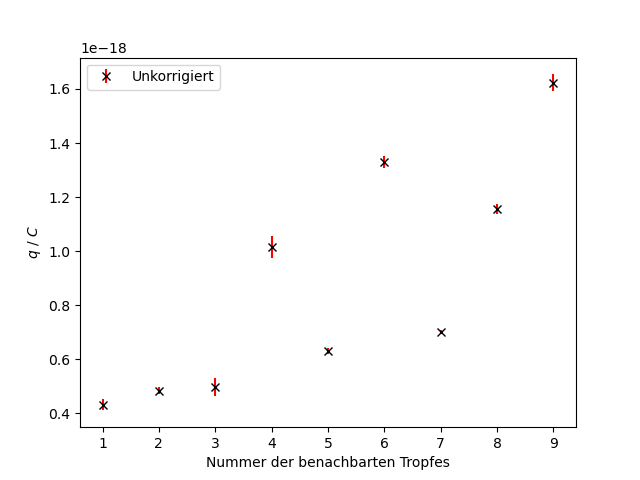
\includegraphics[height=80mm]{bilder/Unkorrigiert.png}
    \caption{Unkorrigierte Ladungen.\label{Abbildung3} }
\end{figure}

\begin{figure}[H]
    \centering
    \includegraphics[height=80mm]{bilder/Korrigiert.png}
    \caption{Korrigierte Ladungen.\label{Abbildung4} }
\end{figure}

\begin{align*}
    \intertext{Dementsprechend folgen für die Elementarladungen}
    e_{0, \text{unkorrigiert}} = (1,749 \pm 0,036) \cdot 10^{-19}\,\unit{\coulomb}\,, \\
    e_{0, \text{korrigiert}}   = (1,651 \pm 0,021) \cdot 10^{-19}\,\unit{\coulomb}\,.
\end{align*}

\begin{figure}[H]
    \centering
    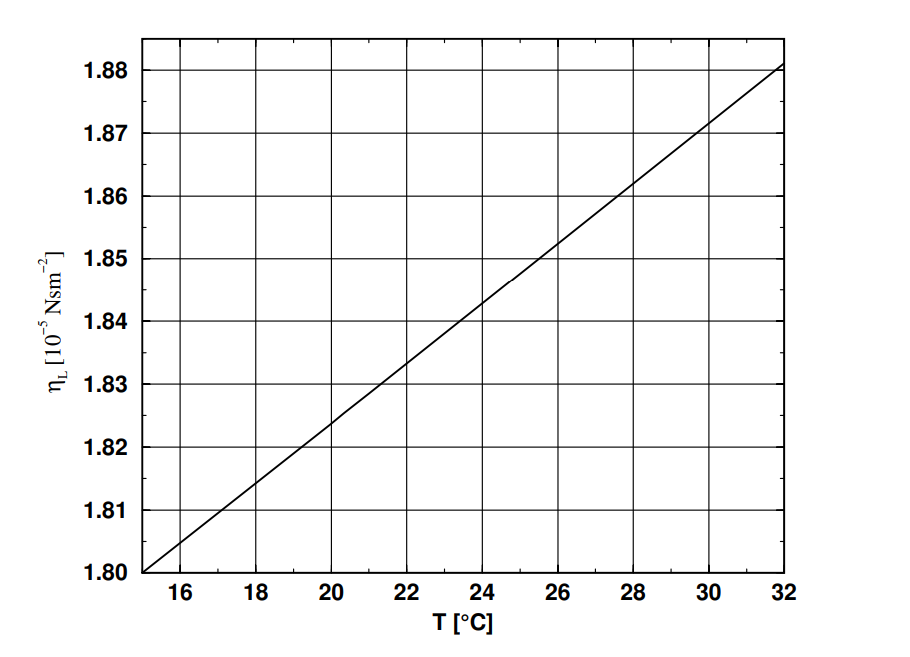
\includegraphics[height=80mm]{bilder/Abb5.png}
    \caption{Viskosität von Luft als Funktion der Temperatur \cite{a1}. \label{Abbildung5} }
\end{figure}

\begin{align}
    \intertext{Aus den gewonnen Ladungen berechnet sich die Avogradokonstante $\text{N}_{\text{a}}$}
    \text{N}_{\text{a}} = \frac{\text{F}}{e_{0}} \label{11}
    \intertext{mit der Faradaykonstante \cite{a4} $\text{F} = 96,485\,\frac{\unit{\coulomb}}{\text{mol}}$.
    Daraus folgt mit den beiden Ladungen $\text{q}_{\text{unkorrigiert}}$ und $\text{q}_{\text{korrigiert}}$: }
    \text{N}_{\text{a, unkorrigiert}} = ( 5,516 \pm 0,113 ) \cdot 10^{23}\,\frac{1}{\text{mol}}\,, \notag \\
    \text{N}_{\text{a, korrigiert}}   = ( 5,844 \pm 0,027 ) \cdot 10^{23}\,\frac{1}{\text{mol}}\,. \notag
\end{align}